\chapter{Experiment}\label{ch:exp}
The experimental procedure is explained in Section \ref{sec:exp.proc}. 
It is discussed what experiments can be done in order to investigate closed-loop stability and the tracking performance of Nonlinear Geometric Control.
In addition, a comparison will be made between the performances of the Nonlinear Geometric Controller and a linear \a{lqr} controller.

The controllers are tested on their ability to track a desired load trajectory. 
Section \ref{sec:exp.traj} presents several desired load trajectories that create different challenges for load position tracking, and it is discussed what could be expected from these experiments.

***************************************\\
Bart: Challenge of what? control challenges?\\
Nam: challenges for load position tracking, beter?

***************************************\\
%in what way a comparison can be made between the performance of the controllers.
%ADD 1 wat brengt mij tot keuze trajectories 
%ADD 2 trajectories
%ADD 3 waar ga ik de resultaten op checken

In Section \ref{sec:exp.setup} the experimental setup is discussed. 
The model parameters for the \a{qr}-Load system are presented, as well as the controller parameters for both Nonlinear Geometric controller and \a{lqr} controller.
The notion of a backstepping command filter is made to explain a mathematical simplification in the experiments.

Finally, in Section \ref{sec:exp.results} the results that are obtained from the load trajectory tracking experiments are presented and discussed.
The stability of the closed-loop system is demonstrated for the Nonlinear Geometric Controller and the differences in linear- and nonlinear controller performance are discussed.

\newpage
\section{Procedure}\label{sec:exp.proc}
Performance of both Nonlinear Geometric Control and \a{lqr} control can be evaluated by comparing their ability to track a load trajectory with minimal error. 
In linear control however, a linearized model is obtained by assuming small angles of both load and \a{qr} around an equilibrium point. 
The model is obtained by assuming the system in equilibrium when the \a{qr} is in hover position with the load hanging directly underneath it.
As a result, the linearized model does not allow direct reference tracking of the load position. 

The \a{lqr} cost function allows control of the inputs $ f $ and $ M $, and the states which define the \a{qr} position, \a{qr} attitude and load attitude. 
Therefore, full load position control is not possible. It can be approached by \a{qr} position control or minimization of the load swing. This limitation illustrates an important difference between the use of a linear and a nonlinear model. 

The experiments describe a smooth desired load trajectory $ x_{L,d}(t) $ in order to get well-defined control functions.
%, which is required to be smooth for Geometric Control, such that feed forward terms can be generated and implemented. 
In this work the desired load paths are generated by hand. The associated required velocity and acceleration are calculated by a \textit{command filter}, which is explained in more detail in Section \ref{sec:exp.setup}.

The experiments done with the \a{lqr} controller will apply reference tracking of the \a{qr} position, which is based on the desired load trajectories that are used for the nonlinear Geometric controller. 
%CHECK 
%DIT MOET ANDERS?
When assuming small angles and minimal load swing, the \a{qr} position should be a cable length above the predefined desired load position. 
Note that this will not allow a direct comparison of the load trajectory tracking performance, nevertheless this will illustrate important differences between the controllers. 
For the purpose of load transportation, both controllers can be used. The difference is in the approach of the problem.

%are defined in a different way.
%with different ob
%in means of
%and allow conclusions to be made about the 
%in load attitude
%exposed to trajectories 
%where large angles are required to track fast maneuvers

% Since it is not possible for \a{lqr} to apply reference tracking for the load trajectory, 
%\a{lqr} is a linear optimal control strategy and will be used to compare its result to a Nonlinear Geometric Controller.

\newcommand{\caseA}{63}
\newcommand{\caseB}{61}
\newcommand{\caseC}{64}
\newpage
\section{Trajectories}\label{sec:exp.traj}
%\begin{description}\label{key}
%\item[Step response] How does the system respond on a smooth step in load trajectory?
%\item[Settling time] How long does it take to stabilize after 
%\end{description}

%What observations can be made in order to adapt the controller properties that improve performance of the test cases.
%ADD
%Description of tests that apply on all cases.

This section discusses a number of cases that describe different load trajectories for the \a{qr}-Load system.
A description is given of desired trajectory and the challenges that are involved.

\subsection*{Case A}
%ADD 
%Explain cases, what can be expected?\\

%\begin{outline}
%	\1 Step Response
%	\2 Settling time (if swing minimization is important)
%	\2 Rise time (important if time critical)
%	\2 Overshoot (if max swing is critical)
%	\2 Steady state error / swing of load (if accuracy is important)
%%	\1 Max load angle
%%	\1 Disturbance Rejection
%	\1 Trajectory tracking
%	\2 How do the errors evolve along the trajectory
%	\2 What is the maximum error during the trajectory
%%	\2 Can we minimize time, while minimizing position error (All Cases)
%%	\2 Minimum position error (All Cases)
%%	\2 Maximum amplitude/frequency of wave with respect to stability (Case B)
%%	\1 Computational Effort (?)
%\end{outline}

%ADD
%why a step function is interesting

%In this first case 
In the first case, a smooth step-like trajectory is generated to investigate the step response of the system.
The step response is a commonly used analysis tool to obtain information about the stability of a dynamical system.
%In a regular step function the system
A step function is used to investigate the effects of a sudden input to the desired load position.
%, such as overshoot, settling time or steady-state value.
%When the controller tries to track the trajectory
Typical response properties that can be investigated are: rise time, overshoot, settling time and steady-state error.
%of the response 
%respond to be investigated are 
%It can be investigated whether the system responds with overshoot or undershoot, the needed settling time and whether the desired steady-state is reached.
The goal is to transport the load from a starting position along the direction of the x-axis to a final position. 
Figure \ref{fig:set.caseA} shows the desired trajectory over time.

The geometric control design requires the desired load trajectory to be twice-differentiable. For this reason a smooth step-like function is generated.
The load position controller outputs a commanded load attitude signal $ q_c $, see Equation \ref{eq:con.q}, 
which is a function of $x_{L,d}, \dot{x}_{L,d} $ and $ \ddot{x}_{L,d} $. 
It can be expected that the step response is only able to track a trajectory up to a limited steepness. 
The commanded acceleration in Equation \ref{eq:con.A} is required to be bounded, such that 
\begin{equation}\label{eq:set.acc}
\parallel (m_Q+m_L)(\ddot{x}_{L,d}+ge_3)+m_QL(\dot{q}\cdot\dot{q})q \parallel < B
\end{equation}
where $ B $ is a design parameter to guarantee Lyapunov stability \cite{Sreenath2013c}. This might result in large errors, and it must be investigated whether the system is able to maintain stable. Input constraints are not yet considered in the control design, this might be required to avoid input commands that are out of reach and 
\begin{figure}[h!]
	\centering
	\makebox[.49\textwidth][c]{\label{fig:AxLd}{\includegraphics[width=.45\textwidth]{\dir{LPOSQRL-xLdes\caseA}}}}
%	\makebox[.49\textwidth][c]{\subfloat[][ \label{fig:AxLdplot}]{\includegraphics[width=.45\textwidth]{\dir{LPOSQRL-xLdesplot\caseA}}}}
	\caption{Desired Load Position Case A\label{fig:set.caseA}}
\end{figure}		

***************************************\\
Bart: Did you found out with Daniel why a steep step works with simple pid controllers?\\
Nam: Waarschijnlijk.. $ e_v $ wordt instantaan oneindig.\\
PID: De gecalculeerde gewenste input wordt instantaan oneindig. De werkelijk response is gelimiteerd door het systeem. Een actuator zal zijn hoogst mogelijke output geven, maar 1 sample periode erna is dat al niet meer nodig, omdat $e_v $ dan weer gezakt is.  \\
NGC: load position controller berekent een commanded load attitude $ q_c=\frac{A}{\parallel A\parallel} $, waar $ A = -k_xe_x-k_ve_v+(m_Q+m_L)(\ddot{x}_{L,d}+ge_3)+m_QL(\dot{q}\cdot\dot{q})q $. 
Als $ e_v \rightarrow\infty$, dan krijg je rotzooi. Het lijkt me dat de controller hierdoor niet meer goed gedefinieërd is. \\
Verderop in een paper staat nog: \textit{Assumed that commanded acceleration is uniformly bounded such that} $\parallel (m_Q+m_L)(\ddot{x}_{L,d}+ge_3)+m_QL(\dot{q}\cdot\dot{q})q\parallel < B $. En dat is niet het geval wanneer er een keiharde step wordt toegepast.

Voorlopige conclusie: \\
PID: controller berekent één sampletijd een oneindig hoge desired input, actuatoren zullen pieken, maar het systeem klapt niet (per se). \\
NGC: load position controller kan geen commanded state meer berekenen voor desired input, waarschijnlijk gaan de control laws hierdoor overhoop. \\
Verder \cite{Bullo2005} geeft een voorbeeld voor trajectory tracking op $ \mathcal{S}^2 $: "Let $ t\mapsto r(t) $ be a twice-differentiable reference trajectory with bounded velocity ...". Wellicht dat met een steile smooth step en een limiet op inputs, dat $ q_c $ (en de rest van de controllers) wel goed gedefinieërd is?

***************************************\\

***************************************\\
Bart: Also speed of response/ rise time is important or not? With high rise time it is easy to have no overshoot but mostly this is not desired behavior.\\
Nam: Edited, please check

***************************************\\

***************************************\\
Bart: You mentioned ""What could be expected from these experiments" --> I don't see the expectation for the step response om this paragraph\\
Nam: Added. Compleet genoeg?

***************************************\\
%ADD inputs f M
%ADD QR attitude
\subsection*{Case B}

%PLANNING: 
%make case to test limits on \a{qr} angles while tracking load trajectory. Is nonlinear GC useful for such aggressive maneuvers?

% BART:
%Enbje wilt dat hellen onderzoelen omdat dat past bij je onderzoeksvraag: agressief manoeuvre en  nonlin

%To investigate the behavior of the system undergoing aggressive maneuvers
The nonlinear geometric controllers are expected to be able to deal with large angles in the \a{qr} attitude, allowing aggressive maneuvering.
This can be tested by describing the next trajectory as a sine wave, growing in amplitude over time, in the direction of one axis in \IF.
This will result in a increasing distance between the load positions at each end of the movement, requiring increasing velocities on both the \a{qr} and the load.
To achieve this, it can be expected that the \a{qr} requires large rotations. It is investigated whether the system is able to perform load position tracking while dealing with increasing \a{qr} rotations.
%attitude needs large angles 
%to fly in a large angle.
%It can be expected that the \a{qr} attitude angles are large to reach the desired velocities.

The trajectory is generated by the product of signals A and B, shown in Figure \ref{fig:set.sinecaseB}, of which the first signal is a sine and the second consists of a smooth step up and down. This product results in signal C, shown in the same figure, which is chosen to be the trajectory in the direction of the y-axis of \IF. Figure \ref{fig:set.xLdcaseB} shows the desired trajectory over time.
\begin{figure}[h!]
	\centering
	\makebox[.49\textwidth][c]{\subfloat[][Trajectory generation\label{fig:set.sinecaseB}]{\includegraphics[width=.45\textwidth]{\dir{LPOSQRL-sineCaseB\caseB}}}}	
	\makebox[.49\textwidth][c]{\subfloat[][Desired trajectory \label{fig:set.xLdcaseB}]{\includegraphics[width=.45\textwidth]{\dir{LPOSQRL-xLdes\caseB}}}}
%	\makebox[.49\textwidth][c]{\subfloat[][ \label{fig:}]{\includegraphics[width=.45\textwidth]{\dir{LPOSQRL-xLdesplot\caseB}}}}
	\caption{Desired Load Position Case B\label{fig:set.caseB}}
\end{figure}			

\subsection*{Case C}
%For this case a
%A trajectory is generated 
This case is generated in order to investigate the response on tracking multiple conditions at the same time.  
%such as sideways position tracking with high velocity, without losing height while tracking up and down motion. 
%this case describes the desired trajectory as follows.
The trajectory along the y-axis in \IF is described as a sine wave with an increasing and decreasing amplitude over time, as in case B.
%, which will require changing and high velocities. 
While following this wave, the load is commanded to move forward along the x-axis, while tracking an increasing and decreasing height.
%has the shape of a sine wave that moves along the y-axis and varies in amplitude in the direction of the x-axis, while 
 %going up and down in the direction of the z-axis.
%Changing velocities are required to track 
The changing amplitude of the trajectory that moves from side to side, requires varying velocities to 'keep up' with the trajectory. 
In this case it can also be expected large \a{qr} rotations are required to track the changing amplitude of the sine wave and the varying velocities.
While doing so, the \a{qr} is expected to lose height due to the rotations, 
It can be investigated how the close-loop system responds to the forward movement, while tracking a swinging motion and whether the controller can correct for the expected height loss, while tracking an up and down movement. 

%movement, while moving forward, up and down.
%How the system reacts on the changes in height
Figure \ref{fig:set.caseC} shows the desired trajectory over time, and a three dimensional representation.
\begin{figure}[h!]
	\centering
	\makebox[.49\textwidth][c]{\subfloat[][\label{fig:}]{\includegraphics[width=.45\textwidth]{\dir{LPOSQRL-xLdes\caseC}}}}
	\makebox[.49\textwidth][c]{\subfloat[][ \label{fig:}]{\includegraphics[width=.45\textwidth]{\dir{LPOSQRL-xLdesplot\caseC}}}}
	\caption{Desired Load Position Case C\label{fig:set.caseC}}
\end{figure}
%CHECK
%Desired load position draaien?

***************************************\\
Bart: Which multiple disciplines? Do you mean Large QR rotations leads to less lifting force which might limit the tracking performance in z-direction\\
Nam: Ik bedoelde eigenlijk, meerdere objectives. Hoge zijwaartse snelheden, terwijl het hoogte moet tracken. Indirect daarmee ook, testen of het hoogte kan houden terwijl de QR kantelt. Beetje herschreven, beter?

***************************************\\
\clearpage		


\section{Setup}\label{sec:exp.setup}
\paragraph{Model parameters}
The simulations are developed using Matlab$^\text{\textregistered} $ and Simulink$^\text{\textregistered} $ R2013b.
The model parameters to define the system are based on a Parrot$^\text{\textregistered} $ Bebop Drone 1, also used in a research by \cite{Cornelis2014}, see Table \ref{tab:set.par}, where $ m_L $ and $ L $ are chosen arbitrarily.
\begin{table}[h!]
	\centering
	\begin{tabular}{|l|ll|l|}
		\hline
		\textbf{Parameter}&\textbf{Value}&&\textbf{Description}\\
		\hline
		$ m_Q $&0.4& $ kg $&Quadrotor Mass\\
		$ l $&0.126& $ m $&Arm length from \a{qr} \a{cm} to rotor\\
		$ I_{xx} $&2.23$ \times 10^{-3}$&$kgm^2 $&Quadrotor Inertia about x-axis\\
		$ I_{yy} $&2.99$ \times 10^{-3}$&$kgm^2 $&Quadrotor Inertia about y-axis\\
		$ I_{zz} $&4.8$ \times 10^{-3}$&$kgm^2 $&Quadrotor Inertia about z-axis\\
		$ m_L $&0.1 &$ kg $&Load Mass\\
		$ L $&0.7 &$ m $& Cable Length\\		
%		$ d $&&&Drag Constant\\
%		$ b $&&&Thrust Constant\\
%		$ c_{\tau_f} $&&& Constant	\\
		\hline		
	\end{tabular}
	\caption{Modeling Parameters}
	\label{tab:set.par}
\end{table}

In order to get a feel for realistic physical limits, these can be based on hardware data, which could be found on the web \footnote{\url{http://blog.parrot.com/2016/01/12/comparison-bebop-2-vs-bebop-drone/}\label{url:set.bebop}}. 
These values are shown in Table \ref{tab:set.par2}, and can be compared with the simulation results, in order to check whether the outcome is in the same order of magnitude of a real physical system.
\begin{table}[h!]
	\centering
	\begin{tabular}{|ll|l|}
		\hline
		\textbf{Value}&&\textbf{Description}\\
		\hline
		13 & $ m/s $&Maximum top speed\\
		2.5& $ m/s $&Maximum vertical speed\\
		30 &$ deg $&Maximum inclination\\
		\hline
	\end{tabular}
	\caption{Hardware Parameters for Bebop Parrot Drone 1}
	\label{tab:set.par2}
\end{table}

%
%***************************************\\
%Bebop 2\\
%500g, 18 m/s, 6 m/s vert, 35 deg
%
%***************************************\\

***************************************\\
Bart: Inclination of what? Is this the same as QR Attitude?\\
Nam: Yes. Just general definition of inclination. Hellingshoek/inclinatie

***************************************\\

% Max lift, 200 g
% Max total force (mQ+mL)*g
% Max f_i = Max total force / 4
% Max torque = 2 * l * max f_i

\paragraph{Command Filtering}
% %ADD Pro Con Command filter
%Easy implementation. Less computational effort.
%Less accurate, because filters high frequency signals.
%CHECK
%Examples from \cite{Farrell2008} and \cite{Djapic2008}. 
A consequence of a backstepping control approach, is that it increases the order of the commanded states. 
The controllers generate control laws that are a function of the commanded signals and their derivatives.
%, which are generated by the controllers in outer loops.
%In the control design, discussed in Chapter \ref{ch:control}, the load attitude controller generates a commanded QR attitude $ R_c $ and its derivative $ \dot{R}_c $. In the same fashion, the load position controller generates a commanded load attitude $ q_c $ and its derivative $ \dot{q}_c $. 
As can be seen in Chapter \ref{ch:control}, the control laws require the values $ R_c, \dot{R}_c, \ddot{R}_c, q_c, \dot{q}_c $ and $ \ddot{q}_c $.
%Calculating the 
Time derivatives of the virtual control variables may be quite complex and the calculation could result in high computational costs.
Instead of analytic differentiation of these terms, which can be tedious, these values can be obtained with the use of a \textit{Command Filter}\cite{Farrell2008,Farrell2005}. 
% %CHECK nodig?
%https://www.researchgate.net/post/Sliding_Mode_Controller_Vs_Backstepping_Controller
The result of a command filter is that the command signal is being pre-filtered by low pass filters and generates an estimation of the derivatives of the commanded signal. Backstepping command filters are implemented to compute $ \dot{R}_c, \ddot{R}_c,\dot{q}_c, \ddot{q}_c,\dot{x}_{L,d}$ and $\ddot{x}_{L,d} $. 
This approach is explained in more detail in \cite{Borra2012}.
%The transfer function of the original commanded input signal $ X_c^o $ and the filtered output $ X_c $ has the form
%\begin{equation}\label{key}
%\frac{X_c(s)}{X_c^o(s)}=H(s)=\frac{\omega_{n1}}{s+\omega_{n1}}\cdot\frac{\omega_{n2}^2}{s^2+2\zeta\omega_{n2}s+\omega_{n2}^2}
%\end{equation}
%Where $ \zeta $ is the damping ratio and $ \omega_n $ the undamped natural frequency. 
%%%CHECK figure niet nodig?
%%See Figure \ref{fig:app.CF}.
%The filter has the following state space representation
%%CHECK waar dit ook alweer vandaan kwam. Reference in Djapic/Farell -> 3e order voor bacterieen ofzo
%\begin{equation}\label{key}
%\begin{aligned}
%\dot{x}_1 &= x_2\\ %dxc
%\dot{x}_2 &= x_3\\ %ddxc
%\dot{x}_3 &= -(2\zeta \omega_{n2}+\omega_{n1})x_3-(2\zeta\omega_{n1}\omega_{n2}+\omega_{n2}^2)x_2-(\omega_{n1}\omega_{n2}^2)(x_1-x_c^o)
%\end{aligned}
%\end{equation}
%where $ x_1 = x_c$, $ x_2 = \dot{x}_c$ and $ x_3 = \ddot{x}_c$, such that $ x_c $ is the filtered output. 
The nonlinear state space representation of this filter is given by
\begin{equation}\label{key}
\begin{bmatrix}
x_c\\
\dot{x}_c
\end{bmatrix}
=
\begin{bmatrix}
q_1\\
q_2
\end{bmatrix}
\end{equation}
\begin{equation}\label{key}
\begin{bmatrix}
\dot{q}_1(t)\\
\dot{q}_2(t)
\end{bmatrix}
=
\begin{bmatrix}
q_2\\
2\zeta\omega_n\left( S_R\left\lbrace \frac{\omega_n^2}{2\zeta\omega_n}\left[ S_M(x_c^o)-q_1\right] \right\rbrace-q_2 \right) 
\end{bmatrix}
\end{equation}
where $ S_M $ and $ S_R $ are functions that can limit the magnitude and rate. The implemented command filter is shown in Figure \ref{fig:set.cf}.
\begin{figure}[h!]
	\centering
	\makebox[\textwidth][c]{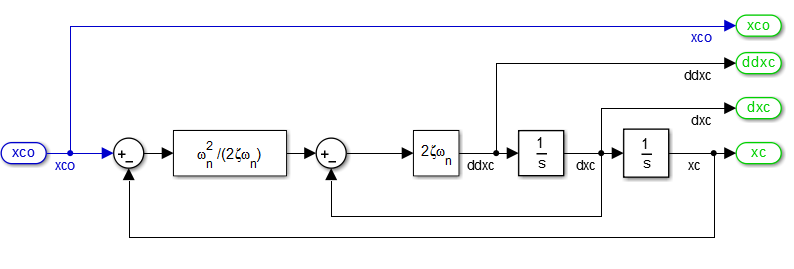
\includegraphics[width=.8\textwidth]{./StyleStuff/CFv2.png}}
	\caption{Command Filter\label{fig:set.cf}}
\end{figure}

The chosen values for $ \omega_n $ and $ \zeta $ for the command filters are shown in Table \ref{tab:set.cf}. 
The parameters were determined by trial and error. 
The higher the value for $ \omega_n $, the higher the frequencies that are passed through the filter. 
Whenever the frequency was chosen too high, noisy derivatives are calculated, resulting in a destabilization of the system.
Choosing the values too low resulted in slow responses, and a bad estimation of the derivatives.
The damping ratio $ \zeta $ was chosen high, in order to give a sufficient damping. No limits for the magnitude and rates are implemented, meaning that $ S_M $ and $ S_R $ are omitted.
\begin{table}[h!]
	\centering
	\caption{Command Filter Parameters}
	\label{tab:set.cf}
\begin{tabular}{|l|lll|}
	\hline
	& \multicolumn{3}{c|}{\textbf{Filter}} \\ \cline{2-4} 
	& $ R  $     & $ q $      & $ x_{L,d} $   \\ \hline
	$ \omega_n $ & 30     & 25     & 25        \\
	$ \zeta  $   & 0.98   & 0.98   & 0.98      \\ \hline
\end{tabular}
\end{table}

% %CHECK  nodig?
%\begin{figure}[h!]
%	\centering
%	\makebox[\textwidth][c]{\includegraphics[width=.45\textwidth]{./StyleStuff/cf.png}}
%	\caption{Representation of the command filter\label{fig:set.CF}}
%\end{figure}		

%The controllers are functions of these commanded signals and their derivatives. Instead of analytic differentiation of these signals, they are obtained by integration by applying a third order low pass filter to the original signals $ R_c^o $ and $ q_c^o $. 
%The state space implementation of this third order filter is \cite{Djapic2008}
%\begin{align}\label{eq:CF}
%\frac{x_c}{x_c^o}&=\frac{\omega_{n1}}{s+\omega_{n1}}\cdot\frac{\omega_{n2}^2}{s^2+2\zeta\omega_{n2}s+\omega_{n2}^2}\\
%\Rightarrow x_c^{'''}&=-(2\zeta\omega_{n2}+\omega_{n1})x_c^{''}-(2\zeta\omega_{n1}\omega_{n2}+\omega_{n2}^2)x_c^{'}-(\omega_{n1}\omega_{n2} ^2)(x_c-x_c^o)
%\end{align}

\paragraph{Geometric Control}
The chosen controller gains in Equations \ref{eq:con.M}, \ref{eq:con.Fpd} and \ref{eq:con.A} can be found in Table \ref{tab:set.gains}.
\begin{table}[h!]
	\centering
	\begin{tabular}{|l|l|l|l|}
		\hline
		%63 61 41
		\textbf{Gain}&\textbf{Case A}&\textbf{Case B}&\textbf{Case C}\\
		\hline
		% % % % % %
		$	k_R	$	&	0.981	&	0.981	&	0.981	\\
		$	k_\Omega	$	&	0.1	&	0.45	&	0.45	\\
		$	k_q	$	&	10	&	10	&	10	\\
		$	k_\omega	$	&	7.5	&	7.5	&	7.5	\\
		$	k_x	$	&	10	&	10	&	10	\\
		$	k_v	$	&	3	&	3	&	3	\\
		% % % % % %	
		\hline
	\end{tabular}
	\caption{Controller Gains Nonlinear Geometric Controller}
	\label{tab:set.gains}
\end{table}

\paragraph{LQR Control}
%ADD why LQR, what is good for / known for
% tuning / easy tuning / 
\acf{lqr} control uses an algorithm to obtain a state-feedback controller, minimizing a cost function depending on the states and weight factors. 
An \a{lqr} design is shown in Figure \ref{fig:set.lqr}
\begin{figure}[h!]
	\centering
	\makebox[\textwidth][c]{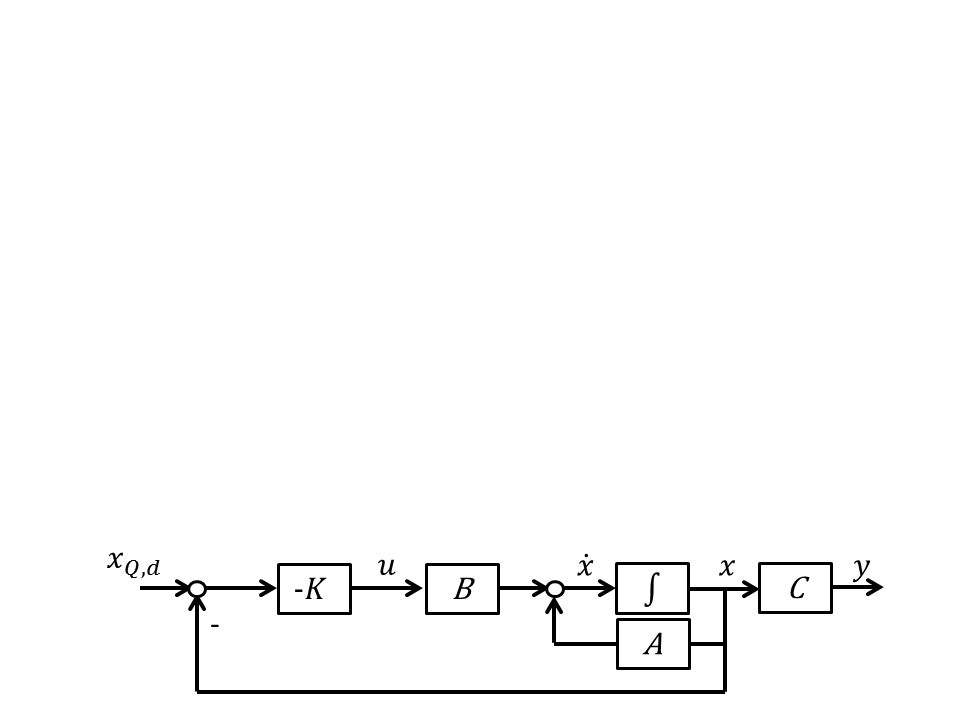
\includegraphics[trim={2cm 0 2cm 14cm},clip,width=.65\textwidth]{./StyleStuff/lqr.png}}
	\caption{LQR control design\label{fig:set.lqr}}
\end{figure}

\a{lqr} control is based on a small angle assumption. 
Therefore, following a traditional modeling method, the rotation matrix is represented with a local coordinate system, 
%Therefore, a traditional modeling method may represent the rotation matrix with a local coordinate system, 
for example with an Euler Angle parameterization. 
A continuous time linearized model of the system used in this controller is represented in the following form 
\begin{align}\label{eq:ss}
\mathbf{\dot{x} }&=A\mathbf{x}+Bu\\
y&=C\mathbf{x}+Du
\end{align}
where $ \mathbf{x} $ is the state vector and $ u $ is the input vector, defined as follows
\begin{align}\label{eq:state}
%	\textbf{x}&=\begin{bmatrix}
%		\textbf{q}\\
%		\mathbf{\dot{q}}
%	\end{bmatrix}\\
%	\mathbf{q}&=\begin{bmatrix}
%		x&y&z&\phi&\theta&\psi&\phi_L&\theta_L
%	\end{bmatrix}^T\\
%	\mathbf{\dot{q}}&=\begin{bmatrix}
%		\dot{x}&\dot{y}&\dot{z}&\dot{\phi}&\dot{\theta}&\dot{\psi}&\dot{\phi}_L&\dot{\theta}_L
%	\end{bmatrix}^T\\
\mathbf{x}&=\begin{bmatrix}
x&y&z&\phi&\theta&\psi&\phi_L&\theta_L&\dot{x}&\dot{y}&\dot{z}&\dot{\phi}&\dot{\theta}&\dot{\psi}&\dot{\phi}_L&\dot{\theta}_L
\end{bmatrix}^T\\
u&=\begin{bmatrix}
f&M_\phi&M_\theta&M_\psi
\end{bmatrix}^T
\end{align}

Using \texttt{Matlab} command \texttt{lqr(A,B,Q,R)}, an optimal gain matrix $ K $ is calculated, such that the state-feedback law $ u=-K(\mathbf{x-x_{ref}}) $ \cite{Reyes-Valeria2013} minimizes the quadratic cost function. Where the cost function is defined as 
\begin{equation}\label{key}
J(u)=\int_{0}^{\infty}(\mathbf{x}^TQ\mathbf{x}+u^TRu)dt
\end{equation}
%where $ Q $ and $ R $ denote weight matrices that penalize the states and inputs in the cost function. 
The weight matrices $ Q $ and $ R $ define the effects of the states and inputs in the cost function, and the gain matrix $K $ can be calculated. 
The derivation of the state space matrices $ A, B, C, D $, the weight matrices $ Q,R $ and the calculated gain matrix $ K $ can be found in Section \ref{app:lqr}. 

\newpage
\section{Results}\label{sec:exp.results}
In this section the results of the experiments are discussed, for each case separately. 
%Figures \ref{fig:set.caseAres}, \ref{fig:set.caseBres} and \ref{fig:set.caseCres} show 
The load tracking performance for the Nonlinear Geometric Controller is discussed by analyzing the desired and actual load trajectories,   
%The desired load trajectories $ x_{L,d} $ and actual load trajectories $ x_L $ are shown, 
together with the corresponding load position and velocity errors.\\
%$ e_x $ and velocity error $ e_v $.\\ 
The stability of the closed-loop system is investigated by observing whether the controller is able to bring the system to a stationary final state.
The error dynamics are analyzed through the error functions, as described in Chapter \ref{ch:control}. 
%Figures \ref{fig:set.caseAres2}, \ref{fig:set.caseBres2} and \ref{fig:set.caseCres2} show 
The configuration errors $ \Psi_R, \Psi_q $
and the corresponding tracking errors of the \a{qr} attitude $ e_R, e_\Omega $, load attitude $ e_q, e_{\dot{q}} $ are presented.\\
%, which can be analyzed to check the system's stability.\\
Finally, the load position tracking results of the Nonlinear Geometric Controller and a \a{lqr} Controller are compared.
%Figures \ref{fig:set.caseAres3}, \ref{fig:set.caseBres3} and \ref{fig:set.caseCres3} show the differences in controller performance.

\subsection*{Case A}
In this case, the desired trajectory was shaped like a smooth step-like function to investigate the response of the system to a sudden input.
The desired and actual load trajectory are shown in Figure \ref{fig:AxL}.
The corresponding load position and velocity error are shown in Figure \ref{fig:AexL}.

Since this function is different from a normal step function, it might be less meaningful to say something about the rise time. 
Normally one checks the time it takes to reach $ 90\% $ of the step height. 
In this case, the step is a smooth function, meaning that the system is not forced to the step height instantly, but in a smooth manner. 
However, it can be seen in Figure \ref{fig:AexLdlqr} that the required time such that $ 90 \% $ of the desired value is reached for the first time is 
%CHECK
$ 0.38 s $.
It can be observed that the system responds with approximately $ 10 \% $ overshoot in the y-direction, and loses height during this maneuver.
This was to be expected due to large \a{qr} rotations. The error remains within a $ 5 \% $ error bound after 
%CHECK
$ 2.83 s $, 
to eventually reach a steady-state at the step size of $ 0.25 m $. 

%ADD
%Also speed of response is important or not? With high rise time it is easy to have no overshoot but mostly this is not desired behavior.\\
%CHECK 
%to increase at a high rate, causing commanded signals to change at high rates. Due to limited bandwidth in the commanded filters, this could cause 

\begin{figure}[h!]
	\centering
	\makebox[.49\textwidth][c]{\subfloat[][]{\includegraphics[width=.49\textwidth]{\dir{LPOSQRL-xL\caseA}}\label{fig:AxL}}}	
	\makebox[.49\textwidth][c]{\subfloat[][]{\includegraphics[width=.49\textwidth]{\dir{LPOSQRL-exL\caseA}}\label{fig:AexL}}}	
	\caption{Load Position Tracking Nonlinear Geometric Control Case A \label{fig:set.caseAres}}
\end{figure}
	

Figure \ref{fig:AeR} and \ref{fig:Aeq} show the tracking errors of the \a{qr} attitude and load attitude, respectively.\\
Observations: $(e_x,e_v,e_q,e_{\dot{q}},e_R,e_\Omega)=(0,0,0,0,0,0) $ is exponentially stable
%The figures show that $ (e_x,e_v)=(0,0) $ is exponentially attractive. 


Figure \ref{fig:APsiR} and \ref{fig:APsiq} show the tracking error functions of the \a{qr} and load, respectively. \\
Observations: there exist constants $ \alpha_q,\beta_q>0 $ such that
\begin{equation}\label{key}
\Psi_q(q(t),q_d(t)) \leq min\left\lbrace 2,\alpha_qe^{-\beta_qt}\right\rbrace 
\end{equation}
\begin{figure}[h!]
	\centering
	\makebox[.49\textwidth][c]{\subfloat[][]{\includegraphics[width=.49\textwidth]{\dir{LPOSQRL-eR\caseA}}\label{fig:AeR}}}	
	\makebox[.49\textwidth][c]{\subfloat[][]{\includegraphics[width=.49\textwidth]{\dir{LPOSQRL-eq\caseA}}\label{fig:Aeq}}}	
	\makebox[.49\textwidth][c]{\subfloat[][]{\includegraphics[width=.49\textwidth]{\dir{LPOSQRL-PsiR\caseA}}\label{fig:APsiR}}}
	\makebox[.49\textwidth][c]{\subfloat[][]{\includegraphics[width=.49\textwidth]{\dir{LPOSQRL-Psiq\caseA}}\label{fig:APsiq}}}
	\caption{Geometric Error functions Nonlinear Geometric Control Case A \label{fig:set.caseAres2}}
\end{figure}	

For both control approaches, Figure \ref{fig:AxLlqr} shows the load position along the desired load position $ x_{L,d} $ and Figure \ref{fig:AexLlqr} shows the load position error. From this can be observed that the \a{lqr} controller has a much slower response. 


Figure \ref{fig:AQRang} shows the \a{qr} attitude with respect to \IF.\\
In Figure \ref{fig:ALang} the load angle with respect to \BF is shown.\\

whereas for the \a{lqr}, this is reached at $  $


\begin{figure}[h!]
	\centering
	\makebox[.49\textwidth][c]{\subfloat[][Load position tracking \label{fig:AxLlqr}]{\includegraphics[width=.49\textwidth]{\dir{LQR-xL\caseA}}}}
	\makebox[.49\textwidth][c]{\subfloat[][Load Position Error\label{fig:AexLlqr}]{\includegraphics[width=.49\textwidth]{\dir{LQR-exL\caseA}}}}	
	\makebox[.49\textwidth][c]{\subfloat[][Load Position Error Percentage\label{fig:AexLdlqr}]{\includegraphics[width=.49\textwidth]{\dir{LQR-exL_xLd\caseA}}}}		
%	\makebox[.49\textwidth][c]{\subfloat[][QR Attitude\label{fig:AQRang}]{\includegraphics[width=.49\textwidth]{\dir{LQR-QRang\caseA}}}}
%	\makebox[.49\textwidth][c]{\subfloat[][Load Attitude\label{fig:ALang}]{\includegraphics[width=.49\textwidth]{\dir{LQR-Lang\caseA}}}}	
	\caption{Controller Comparison Case A. Solid: NGC, Dash-dot: LQR\label{fig:set.caseAres3}}	
\end{figure}
\begin{figure}[h!]
	\centering
%	\makebox[.49\textwidth][c]{\subfloat[][Load position tracking \label{fig:AxLlqr}]{\includegraphics[width=.49\textwidth]{\dir{LQR-xL\caseA}}}}
%	\makebox[.49\textwidth][c]{\subfloat[][Load Position Error\label{fig:AexLlqr}]{\includegraphics[width=.49\textwidth]{\dir{LQR-exL\caseA}}}}	
%	\makebox[.49\textwidth][c]{\subfloat[][Load Position Error Percentage\label{fig:AexLdlqr}]{\includegraphics[width=.49\textwidth]{\dir{LQR-exL_xLd\caseA}}}}		
	\makebox[.49\textwidth][c]{\subfloat[][QR Attitude\label{fig:AQRang}]{\includegraphics[width=.49\textwidth]{\dir{LQR-QRang\caseA}}}}
	\makebox[.49\textwidth][c]{\subfloat[][Load Attitude\label{fig:ALang}]{\includegraphics[width=.49\textwidth]{\dir{LQR-Lang\caseA}}}}	
	\caption{Controller Comparison Case A. Solid: NGC, Dash-dot: LQR\label{fig:set.caseAres4}}	
\end{figure}
\clearpage

\newpage
\subsection*{Case B}
Figure \ref{fig:BxLlqr} shows the load position along the desired load position $ x_{L,d} $ of both controllers.

\begin{figure}[h!]
	\centering
	\makebox[.495\textwidth][c]{\subfloat[][]{\includegraphics[width=.49\textwidth]{\dir{LPOSQRL-xL\caseB}}\label{fig:BxL}}}	
	\makebox[.495\textwidth][c]{\subfloat[][]{\includegraphics[width=.49\textwidth]{\dir{LPOSQRL-exL\caseB}}\label{fig:BexL}}}	
	\caption{Load Position Tracking Nonlinear Geometric Control Case B \label{fig:set.caseBres}}
\end{figure}	

\begin{figure}[h!]
	\centering
	\makebox[.49\textwidth][c]{\subfloat[][]{\includegraphics[width=.49\textwidth]{\dir{LPOSQRL-eR\caseB}}\label{fig:BeR}}}
    \makebox[.49\textwidth][c]{\subfloat[][]{\includegraphics[width=.49\textwidth]{\dir{LPOSQRL-eq\caseB}}\label{fig:Beq}}}	
	\makebox[.49\textwidth][c]{\subfloat[][]{\includegraphics[width=.49\textwidth]{\dir{LPOSQRL-PsiR\caseB}}\label{fig:BPsiR}}}
	\makebox[.49\textwidth][c]{\subfloat[][]{\includegraphics[width=.49\textwidth]{\dir{LPOSQRL-Psiq\caseB}}\label{fig:BPsiq}}}
	\caption{Geometric Error functions Nonlinear Geometric Control Case B \label{fig:set.caseBres2}}
\end{figure}	

%ADD
% Angles QR LOAD?

Figure \ref{fig:BxLlqr} shows the load position along the desired load position $ x_{L,d} $ for both control approaches.\\
Figure \ref{fig:BexLlqr} shows the load position error for both control approaches.

\begin{figure}[h!]
	\centering
	\makebox[.49\textwidth][c]{\subfloat[][Load position tracking \label{fig:BxLlqr}]{\includegraphics[width=.49\textwidth]{\dir{LQR-xL\caseB}}}}
	\makebox[.49\textwidth][c]{\subfloat[][Load Position Error\label{fig:BexLlqr}]{\includegraphics[width=.49\textwidth]{\dir{LQR-exL\caseB}}}}	
	\makebox[.49\textwidth][c]{\subfloat[][QR Attitude\label{fig:BQRang}]{\includegraphics[width=.49\textwidth]{\dir{LQR-QRang\caseB}}}}
	\makebox[.49\textwidth][c]{\subfloat[][Load Attitude\label{fig:BLang}]{\includegraphics[width=.49\textwidth]{\dir{LQR-Lang\caseB}}}}
%	\makebox[.49\textwidth][c]{\subfloat[][Load Position Error Percentage\label{fig:BexLdlqr}]{\includegraphics[width=.49\textwidth]{\dir{LQR-exL_xLd\caseB}}}}	
	\caption{Controller Comparison Case B. Solid: NGC, Dash-dot: LQR\label{fig:set.caseBres3}}
\end{figure}	
\clearpage

\newpage
\subsection*{Case C}
Figure \ref{fig:CxL} shows the desired load position, and Figure \ref{fig:CexL} shows that the error is dominated by the overshoot in the x-direction, due to the fast desired swinging motion. 

While tracking the required \a{qr} attitude, which tilts the \a{qr} to reach the desired velocities in the right direction, it can be seen that the system has difficulties to also maintain the desired height, which can be explained by the fact that the total force will not point upwards if the \a{qr} is tilted. Despite the fact that the \a{qr} is  moving from side to side, the upward force is still controlled to track the desired height. 
\begin{figure}[h!]
	\centering
	\makebox[.495\textwidth][c]{\subfloat[][]{\includegraphics[width=.49\textwidth]{\dir{LPOSQRL-xL\caseC}}\label{fig:CxL}}}	
	\makebox[.495\textwidth][c]{\subfloat[][]{\includegraphics[width=.49\textwidth]{\dir{LPOSQRL-exL\caseC}}\label{fig:CexL}}}	
	\caption{Load Position Tracking Nonlinear Geometric Control Case C \label{fig:set.caseCres}}
\end{figure}	

Figure \ref{fig:CeR} and \ref{fig:Ceq} show the tracking errors of the \a{qr} attitude and load attitude, respectively. \\
Observations: $(e_x,e_v,e_q,e_{\dot{q}},e_R,e_\Omega)=(0,0,0,0,0,0) $ is exponentially stable.
Figure \ref{fig:CPsiR} and \ref{fig:CPsiq} show the tracking error functions of the \a{qr} and load, respectively. \\
Observations: there exist constants $ \alpha_q,\beta_q>0 $ such that
\begin{equation}\label{key}
\Psi_q(q(t),q_d(t)) \leq min\left\lbrace 2,\alpha_qe^{-\beta_qt}\right\rbrace 
\end{equation}
\begin{figure}[h!]
	\centering
	\makebox[.49\textwidth][c]{\subfloat[][]{\includegraphics[width=.49\textwidth]{\dir{LPOSQRL-eR\caseC}}\label{fig:CeR}}}
	\makebox[.49\textwidth][c]{\subfloat[][]{\includegraphics[width=.49\textwidth]{\dir{LPOSQRL-eq\caseC}}\label{fig:Ceq}}}	
	\makebox[.49\textwidth][c]{\subfloat[][]{\includegraphics[width=.49\textwidth]{\dir{LPOSQRL-PsiR\caseC}}\label{fig:CPsiR}}}
	\makebox[.49\textwidth][c]{\subfloat[][]{\includegraphics[width=.49\textwidth]{\dir{LPOSQRL-Psiq\caseC}}\label{fig:CPsiq}}}
	\caption{Geometric Error functions Nonlinear Geometric Control Case C \label{fig:set.caseCres2}}
\end{figure}	

Figure \ref{fig:CxLlqr} shows the load position along the desired load position $ x_{L,d} $ for both control approaches.\\
Figure \ref{fig:CexLlqr} shows the load position error for both control approaches.
OTHER GAINS FOR LQR!\\
Very small penalty on load angle results in swinging load; decreasing load position error, but very bad anti-swing. 
Observations: fact that LQR can not control load position is obvious.\\

Figure \ref{fig:CQRang} shows the \a{qr} attitude with respect to \IF.\\
In Figure \ref{fig:CLang} the load angle with respect to \BF is shown. \\
Observations: Load angles are huge, check results
\begin{figure}[h!]
	\centering
	\makebox[.49\textwidth][c]{\subfloat[][Load position tracking \label{fig:CxLlqr}]{\includegraphics[width=.49\textwidth]{\dir{LQR-xL\caseC}}}}
	\makebox[.49\textwidth][c]{\subfloat[][Load Position Error\label{fig:CexLlqr}]{\includegraphics[width=.49\textwidth]{\dir{LQR-exL\caseC}}}}
	\makebox[.49\textwidth][c]{\subfloat[][QR Attitude\label{fig:CQRang}]{\includegraphics[width=.49\textwidth]{\dir{LQR-QRang\caseC}}}}
	\makebox[.49\textwidth][c]{\subfloat[][Load Attitude\label{fig:CLang}]{\includegraphics[width=.49\textwidth]{\dir{LQR-Lang\caseC}}}}
%	\makebox[.49\textwidth][c]{\subfloat[][Load Position Error Percentage\label{fig:CexLdlqr}]{\includegraphics[width=.525\textwidth]{\dir{LQR-exL_xLd\caseC}}}}		
	\caption{Controller Comparison Case C. Solid: NGC, Dash-dot: LQR\label{fig:set.caseCres3}}
\end{figure}	
\clearpage

\newpage
\section{Conclusion}\label{set:exp.con}
%CHECK 
%What can we learn and conclude from different performance comparisons
%CHECK
%What is its value of nonlinear control compared to linear control

Geometric Mechanics creates a new perspective 

Nonlinear Geometric Control opens a new way of looking into 

Near the equilibrium configuration, the \a{lqr} controller is able to reduce the swing fast and accurate, as can be seen in the results of case A. 
However, the shortcomings of the \a{lqr} controller become evident when it is commanded to track fast trajectories. Following these trajectories continuously requires fast changing movements, far away from the equilibrium configuration. The controller is not able to cope with the fast changing dynamics, resulting in overshoots and slow responses, lagging behind the desired trajectory.

The nonlinear geometric controller depends on feed forward terms that are obtained from the desired trajectories. 
Trajectory generation approaches exist that are able to generate the required desired position, velocity and acceleration by 
however it is possible to compute these with trajectory generating algorithms too.

The controllers are functions of the computed tracking references $ q_c, R_c $ and their derivatives. These terms are approximated by a command filter, which means that the accuracy decreases because high frequency terms are filtered.

%CHECK
%It can be expected that the nonlinear geometric control allows large \a{qr} angles, whereas the \a{lqr} will possible fail to deviate far from the equilibrium point. 


%ADD conclusie 
% over parameter keuze in controllers. Arbitrair, maar wellicht later wel van belang



